\documentclass[tikz]{standalone}

\usepackage{tikz}
\usetikzlibrary{trees}
\usetikzlibrary{shapes}
\usetikzlibrary{positioning}
\usetikzlibrary{arrows.meta}

\tikzset{
    mynode/.style = {circle, ultra thick, draw=black, align=center,fill=yellow!30,font=\ttfamily\bfseries\Large,text=black},
    mynoder/.style = {circle, ultra thick, draw=black, align=center,fill=red!30,font=\ttfamily\bfseries\Large,text=black},
    mynodeb/.style = {circle, ultra thick, draw=black, align=center,fill=blue!30,font=\ttfamily\bfseries\Large,text=black},
    mynodeg/.style = {circle, ultra thick, draw=gray, align=center,fill=gray!05,font=\ttfamily\bfseries\Large,text=gray!20},
    mynodegr/.style = {circle, ultra thick, draw=gray, align=center,fill=gray!05,font=\ttfamily\bfseries\Large,text=red},
    edgen/.style = {-,ultra thick,black},
    edger/.style = {-,ultra thick,red},
    edgeb/.style = {-,ultra thick,blue},
    edgeg/.style = {-,ultra thick,gray},
    edgegd/.style = {-,ultra thick,brown,dashed}, % back
    edgevd/.style = {-,ultra thick,violet,dotted}, % forward
    edgexd/.style = {-,ultra thick,blue,densely dotted}, % traversal
    every picture/.style={/utils/exec={\ttfamily\bfseries}},
    every picture/.style={font issue=\ttfamily\bfseries},
    font issue/.style={execute at begin picture={#1\selectfont}}
}

\newcommand{\R}[1]{\textcolor{red}{#1}}
\newcommand{\B}[1]{\textcolor{violet}{#1}}

\begin{document}

%% 1 Con disuglianza
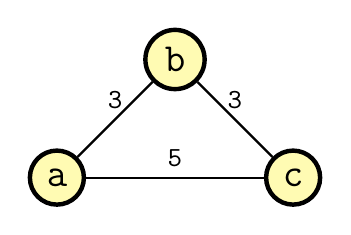
\begin{tikzpicture}[scale=1.00,transform shape]
\node[mynode] at ( 0.00,  0.00) (a) {a};
\node[mynode] at ( 1.50,  1.50) (b) {b};
\node[mynode] at ( 3.00,  0.00) (c) {c};
\draw[edgen, thick,-] (a) edge[above] node {5} (c);
\draw[edgen, thick,-] (a) edge[above] node {3} (b);
\draw[edgen, thick,-] (b) edge[above] node {3} (c);
\end{tikzpicture}

%% 1 Senza disuguaglianza
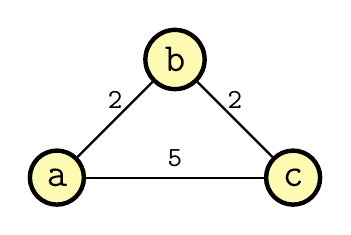
\begin{tikzpicture}[scale=1.00,transform shape]
\node[mynode] at ( 4.50,  0.00) (d) {a};
\node[mynode] at ( 6.00,  1.50) (e) {b};
\node[mynode] at ( 7.50,  0.00) (f) {c};
\draw[edgen, thick,-] (d) edge[above] node {5} (f);
\draw[edgen, thick,-] (d) edge[above] node {2} (e);
\draw[edgen, thick,-] (e) edge[above] node {2} (f);

\end{tikzpicture}

\end{document}